\tikzstyle{decision} = [diamond, draw, fill=blue!20,
    text width=4.5em, text badly centered, node distance=2.5cm, inner sep=0pt]
\tikzstyle{block} = [rectangle, draw, fill=blue!20,
    text width=5em, text centered, rounded corners, minimum height=4em]
\tikzstyle{line} = [draw, very thick, color=black!50]
\tikzstyle{cloud} = [draw, ellipse,fill=red!20, node distance=3cm,
    minimum height=2em]

\newcommand*{\ArrowLength}{2.0em}
\newcommand*{\MyRightArrow}[1][]{
    \tikz [-stealth, red, yshift=0.5ex, baseline] 
        \draw [-stealth, #1] (0,0) -- (\ArrowLength,0) ;
}

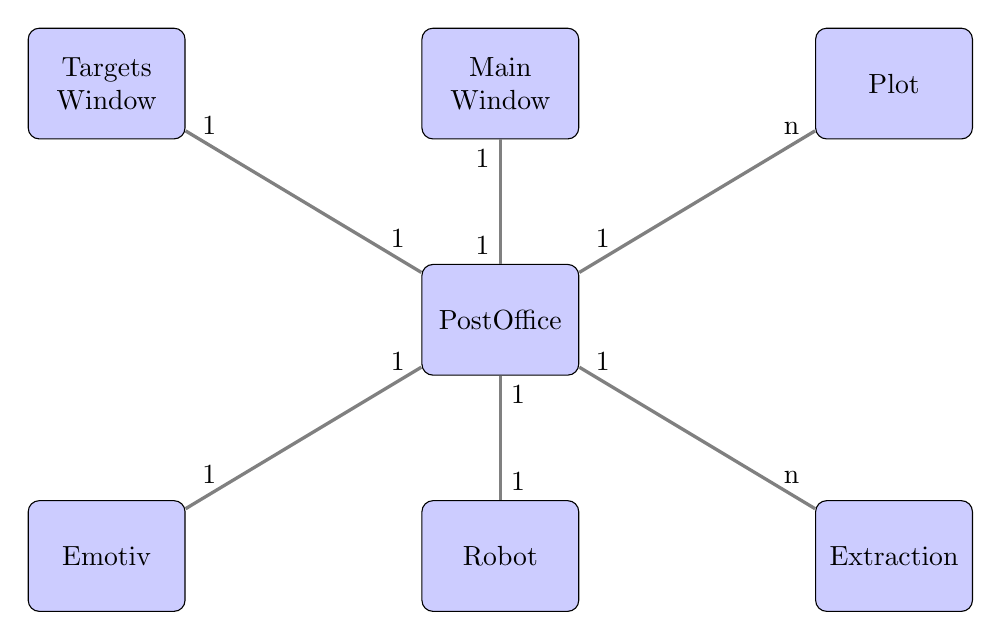
\begin{tikzpicture}[scale=2, node distance = 5cm, auto]
	% Nodes
	\node [block] (PostOffice) {PostOffice};
	\node [block, above of=PostOffice, node distance=3cm] (MainWindow) {Main Window};
	\node [block, left of=MainWindow] (TargetsWindow) {Targets Window};
	\node [block, below of=PostOffice,  node distance=3cm] (Robot) {Robot};
	\node [block, left of=Robot] (MyEmotiv) {Emotiv};
	\node [block, right of=MainWindow] (Plot) {Plot};
	\node [block, right of=Robot] (Extraction) {Extraction};
	
	% Arrows
	\path [line] (PostOffice) -- node [pos=0.1, above, color=black] {1} node[pos=0.9, above, color=black] {1} (MyEmotiv);
	\path [line] (PostOffice) -- node [pos=0.1, above, color=black] {1} node[pos=0.9, above, color=black] {1} (TargetsWindow);
	\path [line] (PostOffice) -- node [pos=0.15, color=black] {1} node[pos=0.85, color=black] {1} (MainWindow);
	\path [line] (PostOffice) -- node [pos=0.15, color=black] {1} node[pos=0.85, color=black] {1} (Robot);
	\path [line] (PostOffice) -- node [pos=0.1, above, color=black] {1} node[pos=0.9, above, color=black] {n} (Plot);
	\path [line] (PostOffice) -- node [pos=0.1, above, color=black] {1} node[pos=0.9, above, color=black] {n} (Extraction);

\end{tikzpicture}
